\documentclass{article}

\textwidth=6.5in
\textheight=8.5in
\voffset=-54pt
\oddsidemargin=0in
\evensidemargin=0in
\setlength{\parskip}{8pt}
\setlength{\parindent}{0pt}

\usepackage{workbook}

\usepackage{handout}

\usepackage{exam}

\newcommand{\answerbox}[3][]{
    \fbox{\begin{minipage}[t][#2][c]{#3}
        #1
    \end{minipage}}
    }

\begin{document}

{\large \mbox{} \hfill \bf Name:\underline{\hspace{3in}}}\\[2pt]
{\mbox{} \hfill \it (Please write your name neatly in print.)}\\[12pt]
{\large \mbox{} \hfill \bf HUID:\underline{\hspace{3in}}}
 
\medskip
 
\noindent
{\large\bf
Final Exam Practice 2\\
Math Mb Spring 2025}
\noindent


{\Large
\begin{center}\textbf{Directions---Please read carefully!} \end{center}}

This is a practice test. The same directions will appear on the actual exam, so read them carefully.

\hrulefill 


This exam is subject to the Harvard College Honor Code. No calculators or any other aids are permitted.  Please write as neatly as possible, as answers that can't be read can't be graded and thus can't receive credit. To receive full credit, you must show relevant working
and include units when appropriate. 

You have 180 minutes to complete this exam. 

You may ask for scratch paper if you need additional space to write, but it will not be scanned or graded. Make sure to include all relevant working in this exam booklet in the space provided for each question.

\begin{center}\textbf{Good luck!}\end{center}


\vfill

\centering{
\emph{As a member of Harvard College, I pledge that I will not give or receive assistance on this exam.}}
\vspace{0.3in}

{\large \mbox{} \hfill \bf Signature:\underline{\hspace{3in}}}
\thispagestyle{empty}

\newpage

\begin{enumerate}
\item
  \label{spring2011-midterm1-3-modified}
  
  Scientists analyzing data on carbon emissions at a factory say the
  emissions at time $t$ are well-approximated by the function $f(t)=3\sin
  (2t) + 3\sqrt 3\, t $.

  \begin{enumerate}
  \item 
    \begin{problem}[\vfill]
      Find the absolute minimum value of $f(t)$ on the
      interval $\left[0, 2 \pi \right]$.
    \end{problem}

    \begin{solution}
      \ideas{We'll start by finding the points where $f'(t) = 0$.}
      We want to solve:
      \begin{align}
        f'(t) &= 0 \nonumber \\
        3 \cos(2t) \cdot 2 + 3 \sqrt{3} &= 0 \nonumber \\
        6 \cos (2t) &= -3 \sqrt{3} \nonumber \\
        \cos(2t) &= -
        \frac{\sqrt{3}}{2} \label{spring2011-midterm1-3-eq1} 
      \end{align}
      We want to solve this on $\left[0, 2 \pi \right]$.  Let's
      substitute $u = 2t$; values of $t$ between $0$ and $2 \pi$
      correspond to values of $u$ in $[0, 4 \pi]$, so we first want to:
      \begin{center}
        Solve $\cos u = - \frac{\sqrt{3}}{2}$ on $[0, 4 \pi]$.
      \end{center}
      There are 4 solutions, $u = \displaystyle \frac{5 \pi}{6}, \frac{7
        \pi}{6}, \frac{17 \pi}{6}, \frac{19 \pi}{6}$.

      Now, we can go back and solve for $t$: since $u = 2t$, $t =
      \frac{u}{2}$, so the solutions are $t = \frac{5 \pi}{12}, \frac{7
        \pi}{12}, \frac{17 \pi}{12}, \frac{19 \pi}{12}$.

      \ideas{But these are just the points where $f'(t) = 0$; we still
        need to figure out where the absolute minimum and maximum are.
        Because we have a lot of points where $f'(t) = 0$, an effective
        strategy is to just plug each into $f$ and check the endpoints.}

      Next, we plug these values, as well as the endpoints $0$ and
      $2 \pi$, into $f$ to see which gives us the lowest value:
      \begin{align*}
        f(0) &= 3 \sin (0) + 3 \sqrt{3} \cdot 0 = 0 \\
        f \left( \frac{5 \pi}{12} \right) &= 3 \sin \frac{5 \pi}{6} + 3
        \sqrt{3} \cdot \frac{5 \pi}{12} = \frac{3}{2} + \frac{5 \sqrt{3}
          \pi}{4} \\
        f \left( \frac{7 \pi}{12} \right) &= 3 \sin \frac{7 \pi}{6} + 3
        \sqrt{3} \cdot \frac{7 \pi}{12} = - \frac{3}{2} + \frac{7 \sqrt{3}
          \pi}{4} \\
        f \left( \frac{17 \pi}{12} \right) &= 3 \sin \frac{17 \pi}{6} + 3
        \sqrt{3} \cdot \frac{17 \pi}{12} = \frac{3}{2} + \frac{17 \sqrt{3} 
          \pi}{4} \\
        f \left( \frac{19 \pi}{12} \right) &= 3 \sin \frac{19 \pi}{6} + 3
        \sqrt{3} \cdot \frac{19 \pi}{12} = - \frac{3}{2} + \frac{19
          \sqrt{3} \pi}{4} \\
        f(2 \pi) &= 3 \sin (4 \pi) + 3 \sqrt{3} \cdot 2 \pi = 6 \sqrt{3}
        \pi 
      \end{align*}
      Looking at these, we can see that all but $f(0)$ are positive, so
      $f(0) = 0$ is the minimal value.  Therefore, the \fbox{absolute
        minimum value of $f(t)$ on the interval $\left[ 0, 2 \pi \right]$
        is 0}.

\iffalse
      So, now we need to figure out which value is the highest.  It's
      clear that $f \left( \frac{17 \pi}{12} \right) > f \left( \frac{5
          \pi}{12} \right)$ and $f \left( \frac{19 \pi}{12} \right) > f
      \left( \frac{7 \pi}{12} \right)$.  It's also clear that $f (2 \pi) >
      f \left( \frac{19 \pi}{12} \right)$.  So, we really just need to
      decide whether $f \left( \frac{17 \pi}{12} \right)$ or $f(2 \pi)$ is
      greater.
      \begin{align*}
        \frac{3}{2} + \frac{17 \sqrt{3} \pi}{4} & \stackrel{?}{<} 6
        \sqrt{3} \pi \\
        \intertext{Multiply both sides by $4$ to make the comparison
          easier:}
        6 + 17 \sqrt{3} \pi & \stackrel{?}{<} 24 \sqrt{3} \pi \\
        \intertext{Subtract $17 \sqrt{3} \pi$ from both sides to make the
          comparison easier:}
        6 & \stackrel{?}{<} 7 \sqrt{3} \pi 
      \end{align*}
      The right side is clearly bigger (both $\sqrt{3}$ and $\pi$ are
      greater than 1, so the right side is at least 7).  Therefore, $f (2
      \pi)$ is the largest value, so the \fbox{absolute maximum value of
        $f(t)$ on $[0, 2 \pi]$ is $6 \sqrt{3} \pi$}.

      \begin{checkanswer}
        A good check for equation (\ref{spring2011-midterm1-3-eq1}) is
        to think about the graph of $\cos(2t)$; you should know what
        this looks like, and the graph confirms that $\cos(2t) = -
        \frac{\sqrt{3}}{2}$ should have 4 solutions in $[0, 2 \pi]$.
      \end{checkanswer}
\fi
    \end{solution}

  \item    
    Which of the following best describes the long-term behavior of the
    emissions?  (Circle your choice; no explanation is necessary.)
    \begin{enumerate}[label=\protect\maybecircle{\Alph*.}]
    \plainitem The emissions vary periodically over time.
    \plainitem The emissions are always increasing over time.
    \circleitem The emissions fluctuate over time, but the overall trend
      is increasing.
    \end{enumerate}

    \begin{solution}
      The term $3 \sqrt{3} t$ is linear (and increasing), while the term
      $3 \sin (2t)$ just fluctuates between $-3$ and $3$.  Thus, the sum
      $3 \sin(2t) + 3 \sqrt{3} t$ fluctuates between $3 \sqrt{3} t - 3$
      and $3 \sqrt{3} t + 3$:
      \begin{center}
        \begin{tikzpicture}
          \begin{axis}[width=3in, cycle list name=mycolor, clip=false]
            \addplot+[domain=0:31]{3*sin(deg(2*x))+3*sqrt(3)*x}
            node[anchor=south west]{$y = f(t)$};
            \addplot+[domain=0:31]{3*sqrt(3)*x-3} node[pos=0.8,
            anchor=north west] {$y = 3 \sqrt{3} t - 3$};
            \addplot+[domain=0:31]{3*sqrt(3)*x+3} node[pos=0.8,
            anchor=south east] {$y = 3 \sqrt{3} t + 3$};
          \end{axis}
        \end{tikzpicture}
      \end{center}
      \emph{Note:} We know that $f(t)$ isn't always increasing because we
      found local extrema in the previous part. 
    \end{solution}

    \pspace{0.35in}
  \end{enumerate}

  \pspace{\newpage}

\item \label{spring2010-final-review-1}

  Suppose that the function $r(t)$, given by the graph below, models the
  rate at which your stock portfolio is gaining (or losing) value,
  measured in dollars per month, where $t = 0$ corresponds to January 1,
  2010 and $t$ is measured in months.  On February 1, 2010, the portfolio
  was worth \$1000.

  \begin{tabular}{c}
    $r(t) = $ rate at which your stock portfolio is \\
    gaining/losing value
    (dollars per month) \\[18pt]
    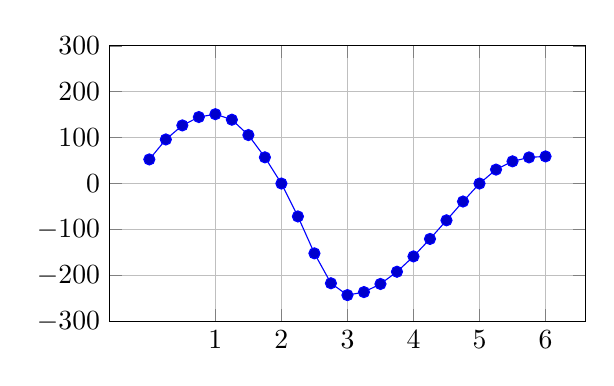
\begin{tikzpicture}[declare function={
        f(\x) = and(0 <= \x, \x <=1.0073) * (52.55474452554742 + 200.0000000000001*\x - 105.74984247006972*\x^2 + 4.285042418929447*\x^3)
        + and(1.0073 < \x, \x <=2) * (-143.03571693236768 + 653.2779891267917*\x - 427.43831188570965*\x^2 + 68.27912327770284*\x^3)
        + and(2 < \x, \x <=2.9927) * (-2625.0989791927636 + 3887.457448211955*\x - 1800.0703242755771*\x^2 + 256.3081724838951*\x^3)
        + and(2.9927 < \x, \x <=5) * (1318.359095150506 - 1247.7159520802898*\x + 310.82251330196436*\x^2 - 22.802737338385324*\x^3)
        + and(5 < \x, \x <=6) * (-7839.37003372821 + 3786.8367673800803*\x - 604.0710790167383*\x^2 + 32.05570537797013*\x^3)
        ;}]
      \begin{axis}[grid=major, ymin=-300, ymax=300, ytick={-300, -200, ...,
          300}, width=3in, height=2in, xtick={1, 2, ..., 6}]
        \addplot+[domain=0:6] {f(x)};
      \end{axis}
    \end{tikzpicture}
  \end{tabular}

  \begin{enumerate}

  \item
    \begin{problem}[\vfill]
      Write an expression involving a definite integral which gives the
      total value of your stock portfolio at the start of April ($t =3$).
    \end{problem}

    \begin{solution}
      We are told that, at $t = 1$, the portfolio is worth 1000.  From $t
      = 1$ to $t = 3$, the value of the portfolio changes by
      $\displaystyle \int_1^3 r(t)\,dt$.  Thus, the value of the portfolio
      at $t = 3$ is $\boxed{1000 + \int_1^3 r(t)\,dt}$. 
    \end{solution}

  \item
    \begin{problem}[\vfill]
      At what times in $(0, 6)$ was your stock portfolio increasing in
      value?
    \end{problem}

    \begin{solution}
      Since $r(t)$ gives the rate of change (i.e., derivative) of the
      value, the value is increasing whenever $r(t)$ is positive, which
      happens on \fbox{$(0, 2)$ and $(5, 6)$}.
    \end{solution}

  \item
    \begin{problem}[\vfill]
      Between January 1 and July 1, at what time was your stock portfolio
      worth the most?
    \end{problem}

    \begin{solution}
      In the previous part, we determined that the value of the portfolio
      increases on $(0, 2)$, decreases on $(2, 5)$, and increases again on
      $(5, 6)$. Therefore, your stock portfolio must be worth the most at
      either $t = 2$ or $t = 6$.  The stock's value at $t = 2$ is $1000 +
      \displaystyle \int_1^2 r(t)\,dt$, and the stock's value at $t = 6$
      is $1000 + \displaystyle \int_1^6 r(t)\,dt$.  From the graph of
      $r(t)$, we can see that $\displaystyle \int_1^2 r(t)\,dt > \int_1^6
      r(t)\,dt$, so the stock is worth the most at $\boxed{t = 2}$, or
      \fbox{the beginning of March}.
    \end{solution}
    
\pspace{\newpage}

  \item \label{spring2010-final-review-1-sketch-value-graph} 
    \begin{problem}[\stretch{4}]
      Sketch a graph of the value of your portfolio between January and
      July.  Your graph does not have to be exact, but it should
      accurately reflect where the graph is increasing/decreasing and
      concave up/concave down.  Please label at least one point on your
      graph with exact coordinates. 
    \end{problem}

    \begin{solution}
      We'd like to sketch the graph of $V(t)$, the value of your portfolio
      at time $t$.  We are given the graph of $r(t)$, which is the
      derivative of $V(t)$.  Therefore, we have the relationships:
      \begin{center}
        \begin{tabular}{l l l}
          $V(t)$ & $r(t) = V'(t)$ \\
          \hline
          increasing & positive \\
          \hline
          decreasing & negative \\
          \hline
          concave up & increasing \\
          \hline
          concave down & decreasing
        \end{tabular}
      \end{center}
      Looking at the graph of $r(t)$, we can figure out the intervals on
      which each property holds:
      \begin{center}
        \begin{tabular}{l l l}
          $V(t)$ & $r(t) = V'(t)$ & true on intervals \\
          \hline
          increasing & positive & $(0, 2), (5, 6)$\\
          \hline
          decreasing & negative & $(2, 5)$ \\
          \hline
          concave up & increasing & $(0, 1), (3, 6)$ \\
          \hline
          concave down & decreasing & $(1, 3)$
        \end{tabular}
      \end{center}
      In addition, we are told that $V(1) = 1000$. So, we get the
      following rough graph:
      \begin{center}
        \begin{tikzpicture}[declare function={f(\x)=
            (\x < 1) * (-118.37605764025659 + 52.55474452554741*x + 100.00000000000006*x^2 - 35.24994749002324*x^3 + 1.0712606047323618*x^4) +
            and(1 <= \x, \x < 2) * (-58.193604477197454 - 143.0357169323677*x + 326.63899456339584*x^2 - 142.47943729523658*x^3 + 17.06978081942571*x^4) +
            and(2 <= \x, \x < 2.9927) * (1345.8098380881447 - 2625.0989791927636*x + 1943.7287241059776*x^2 - 600.0234414251923*x^3 + 64.07704312097376*x^4) +
            and(2.9927 <= \x, \x < 5) * (-722.3237493256918 + 1318.359095150506*x - 623.8579760401448*x^2 + 103.60750443398813*x^3 - 5.700684334596332*x^4) +
            (\x >= 5) * (11683.347573995341 - 7839.37003372821*x + 1893.41838369004*x^2 - 201.35702633891276*x^3 + 8.013926344492532*x^4);}]
          \begin{axis}[ymin=0, ytick={1000}, width=3in, height=2in,
            xtick={1, 2, ..., 6}]
            \addplot+[domain=0:6] {f(x) + 1000};
            \addplot+[closed] coordinates { (1, 1000) } node[anchor=north
            west] {$(1, 1000)$};
          \end{axis}
        \end{tikzpicture}
      \end{center}
    \end{solution}

  \item 
    \begin{problem}[\stretch{1}]
      On the graph you sketched in
      \ref{spring2010-final-review-1-sketch-value-graph}, sketch the graph
      of the function $\displaystyle  A(t) =  \int_3^t r(x)\,dx$.
      Please label at least one point with exact coordinates. 
    \end{problem}

    \begin{solution}
      By FTOC 1, $A'(t) = r(t)$.  In words, $A(t)$ is an
      antiderivative of $r(t)$.  But the function $V(t)$ we sketched in
      \ref{spring2010-final-review-1-sketch-value-graph} is also an
      antiderivative of $r(t)$, and any two antiderivatives of $r(t)$ must
      differ by a constant.  That is, $A(t)$ can be expressed as
      $V(t) + C$ for some constant $C$, so the graph of $A(t)$ is
      simply a vertical shift of $V(t)$.  But how far do we shift?  Well,
      we know $A(3) = 0$, so we shift $V(t)$ down until we get a
      graph which has $3$ as a $t$-intercept: 
      \begin{center}
        \begin{tikzpicture}[declare function={f(\x)=
            (\x < 1) * (-118.37605764025659 + 52.55474452554741*x + 100.00000000000006*x^2 - 35.24994749002324*x^3 + 1.0712606047323618*x^4) +
            and(1 <= \x, \x < 2) * (-58.193604477197454 - 143.0357169323677*x + 326.63899456339584*x^2 - 142.47943729523658*x^3 + 17.06978081942571*x^4) +
            and(2 <= \x, \x < 2.9927) * (1345.8098380881447 - 2625.0989791927636*x + 1943.7287241059776*x^2 - 600.0234414251923*x^3 + 64.07704312097376*x^4) +
            and(2.9927 <= \x, \x < 5) * (-722.3237493256918 + 1318.359095150506*x - 623.8579760401448*x^2 + 103.60750443398813*x^3 - 5.700684334596332*x^4) +
            (\x >= 5) * (11683.347573995341 - 7839.37003372821*x + 1893.41838369004*x^2 - 201.35702633891276*x^3 + 8.013926344492532*x^4);}]
          \begin{axis}[ytick={1000}, width=3in, height=2in,
            xtick={1, 2, ..., 6}]
            \addplot+[domain=0:6] {f(x) + 1000};
            \addplot+[domain=0:6, blue] {f(x) + 46.3211};
            \addplot+[closed] coordinates { (1, 1000) } node[anchor=north
            west] {$(1, 1000)$};
            \addplot+[closed, blue] coordinates { (3, 0) } node[anchor=south
            west] {$(3, 0)$};
          \end{axis}
        \end{tikzpicture}
      \end{center}      
    \end{solution}
  \end{enumerate}

  \pspace{\newpage}

\item \label{spring2011-midterm1-revisit-8-extended}

  Below is a picture of the curve $\displaystyle \left( \frac{x}{2} + y
  \right)^4 = 8xy$.

\begin{center}
   
\includegraphics[width=2in]{Final Exam/Practice Exams/implicit-curve-skewed-figure-8.pdf}
   \end{center}

  \begin{enumerate}
  \item \label{spring2011-midterm1-revisit-8a}
    \begin{problem}[0.25in]
      Find the equation of the line tangent to the curve at the point $(2,
      1)$.

     
    \end{problem}

\probonly{\vspace{2in}}
    \begin{problemonly}
        \emph{Check that your answer seems reasonable given the picture.}
      \end{problemonly}

    \begin{solution}
      The slope of the tangent line we want is $\dfrac{dy}{dx}$ at the
      point $(2, 1)$; let's find this using implicit differentiation.  We
      start with the given equation:
      \begin{align*}
        \left( \frac{x}{2} + y \right)^4 &= 8xy \\
        \intertext{Differentiate both sides with respect to $x$:}
        \frac{d}{dx} \left(\fcolorbox{red}{white}{$\displaystyle
            \fcolorbox{blue}{white}{$\displaystyle \left(\frac{x}{2}+
                y\right)$}^ { 4} $}\right) &= \frac{d}{dx}
        \left(\fcolorbox{purple}{white}{$\displaystyle 8$}\cdot x\cdot
          y\right) \\
        4 \left(\frac{x}{2}+ y\right)^ { 3} \cdot
        \frac{d}{dx}\left(\frac{x}{2}+ y\right) &= 8\cdot \frac{d}{dx}
        \left(\fcolorbox{green}{white}{$\displaystyle x$}\cdot
          \fcolorbox{green}{white}{$\displaystyle  y$}\right) \\
        4 \left(\frac{x}{2}+ y\right)^ { 3} \cdot \left(\frac{1}{2}+
          \frac{dy}{dx} \right) &= 8 \left(x\cdot
          \frac{dy}{dx} + y\right) \\
        \intertext{Since we only care about what happens at the point $(2,
          1)$, we can plug in $x = 2, y = 1$:} 32 \left( \frac{1}{2} +
          \frac{dy}{dx} \right) &= 8 \left(
          2 \frac{dy}{dx} + 1 \right) \\
        \intertext{We want to solve for $\dfrac{dy}{dx}$:}%
        16 + 32 \frac{dy}{dx} &= 16 \frac{dy}{dx} + 8 \\
        16 \frac{dy}{dx} &= -8 \\
        \frac{dy}{dx} &= - \frac{1}{2}
      \end{align*}
      So, the slope of the tangent line we're looking for is
      $-\dfrac{1}{2}$.  The line contains the point $(2, 1)$, so its
      equation is $\boxed{y - 1 = - \frac{1}{2} (x - 2)}$.

      \begin{checkanswer}
        From the picture, it looks like the tangent line should have
        negative slope, so our answer seems reasonable.
      \end{checkanswer}
    \end{solution}

  \item
    \begin{problem}[\vfill]
      Use linear approximation to approximate the $y$-coordinate of the
      point on the curve near $(2, 1)$ whose $x$-coordinate is 1.9.
    \end{problem}


    \begin{problemonly}
        \emph{Check that your answer seems reasonable given the picture.}
        \newpage
      \end{problemonly}

    \begin{solution}
      Near $(2, 1)$, the line $y - 1 = - \frac{1}{2} (x - 2)$ should be
      very close to the graph of the actual curve $\displaystyle \left(
        \frac{x}{2} + y \right)^4 = 8xy$.  So, the point on the
      \emph{line} with $x$-coordinate $1.9$ should be a good approximation
      for the point on the \emph{curve} with $x$-coordinate $1.9$.  The
      line can be written as $y = 1 - \frac{1}{2} (x - 2)$, so when $x =
      1.9$, $y = 1.05$ (that is, $(1.9, 1.05)$ is a point on the line).
      So, $\boxed{1.05}$ should be a good estimate for the $y$-coordinate
      of the point on the curve we're interested in.

      \begin{checkanswer}
        From the picture, we can see that the $y$-coordinate we're talking
        about ought to be just a bit higher than $1$, so our answer seems
        reasonable.
      \end{checkanswer}
    \end{solution}
\end{enumerate}

Problem 3 continues here: $\displaystyle \left( \frac{x}{2} + y
  \right)^4 = 8xy$
  
\begin{center}
   
\includegraphics[width=2in]{Final Exam/Practice Exams/implicit-curve-skewed-figure-8.pdf}
   \end{center}

\begin{enumerate}[resume]
  
  \item
    \begin{problem}
      Marita is running on a track shaped like this curve.  At the precise
      instant when she goes through the point $(2, 1)$, her $x$-coordinate
      is increasing at an instantaneous rate of 3 units per minute.  At
      this instant, is her $y$-coordinate increasing or decreasing?  At
      what rate?
    \end{problem}

    \begin{solution}
      \ideas{This is a related rates question; we are asked to find a
        rate, and we are told another rate.  So, let's use our usual
        strategy.  We already have a picture of the curve, so let's figure
        out what we know and what we want to know.}

      \highlight{
        \textbf{What we know:} $\dfrac{dx}{dt} = 3$        

        \textbf{What we want to know:} $\dfrac{dy}{dt}$
      }

      \ideas{Now, we try to relate variables.  In this case, since the
        rate we know about is $\frac{d\bm{x}}{dt}$, and the rate we want
        to know is $\frac{d\bm{y}}{dt}$, we try to relate $x$ and $y$.}

      The variables $x$ and $y$ are related by the equation of the curve:
      \[ \left( \frac{x}{2} + y \right)^4 = 8xy.\]
      \ideas{Now, we can differentiate our relating equation.  Since we
        are looking for $\frac{dy}{d\bm{t}}$, we should differentiate both
        sides with respect to $t$:}        
      \begin{align*}
        \frac{d}{dt} \left(\fcolorbox{red}{white}{$\displaystyle
            \fcolorbox{blue}{white}{$\displaystyle  \left(\frac{x}{2}+
                y\right)$}^ { 4} $}\right) &= \frac{d}{dt}
        \left(\fcolorbox{purple}{white}{$\displaystyle 8$}\cdot x\cdot
          y\right) \\
        4 \left(\frac{x}{2}+ y\right)^ { 3} \cdot
        \frac{d}{dt}\left(\frac{x}{2}+ y\right) &= 8\cdot \frac{d}{dt}
        \left(\fcolorbox{green}{white}{$\displaystyle  x$}\cdot
          \fcolorbox{green}{white}{$\displaystyle  y$}\right) \\ 
        4 \left(\frac{x}{2}+ y\right)^ { 3} \cdot \left(\frac{1}{2}\cdot
          \frac{dx}{dt}+ \frac{dy}{dt}\right) &= 8 \left(x\cdot
          \frac{dy}{dt}+ \frac{dx}{dt}\cdot y\right) \\
        \intertext{Now, we can fill in the information at the time we care
          about: $x = 2$, $y = 1$, and $\dfrac{dx}{dt} = 3$:}
        32 \left( \frac{3}{2} + \frac{dy}{dt} \right) &= 8 \left( 2
          \frac{dy}{dt} + 3 \right) \\
        \intertext{Finally, we solve for $\frac{dy}{dt}$:}
        48 + 32 \frac{dy}{dt} &= 16 \frac{dy}{dt} + 24 \\
        16 \frac{dy}{dt} &= - 24 \\
        \frac{dy}{dt} = - \frac{3}{2}
      \end{align*}
      That is, \fbox{Marita's $y$-coordinate is decreasing at an
        instantaneous rate of $1.5$ units per minute}.

      (Checking with our picture, it makes sense that, if Marita is at
      $(2, 1)$ and her $x$-coordinate is increasing, then her
      $y$-coordinate is decreasing.)

      \emph{Alternate solution:} Here is another way you could have solved
      the problem.  This method takes advantage of what we found in
      \ref{spring2011-midterm1-revisit-8a}.

      We know $\frac{dx}{dt}$, and we are looking for $\frac{dy}{dt}$.  By
      the Chain Rule,
      \begin{align*}
        \frac{dy}{dt} &= \frac{dy}{dx} \frac{dx}{dt} \\
        \intertext{In \ref{spring2011-midterm1-revisit-8a}, we already
          computed $\dfrac{dy}{dx}$ at the point $(2, 1)$ and found that
          it was $- \frac{1}{2}$.  So, we can plug this in:}
        \frac{dy}{dt} &= - \frac{1}{2} \cdot 3 = - \frac{3}{2}
      \end{align*}
    \end{solution}

  \end{enumerate}
  \probonly{\newpage}

\item
  \label{francois-rope-optimization} % Carl Erickson

  There is a rope stretched out in front of Fran\c{c}ois.  The point on
  the rope closest to Fran\c{c}ois is 100 meters away from him, and he is
  facing this point.  Call this point $P$.  There are two knots tied in
  the rope: knot $A$ is 6 meters to the left of point $P$ and knot $B$ is
  $5$ meters to the left of point $P$.  (See the diagram below, which is
  not to scale.)
  \begin{center}
    \begin{tikzpicture}[scale=0.75]
      \draw (-7, 0) -- (7, 0);
      \filldraw (0, 0) node[above] {$P$} circle (1.5pt);
      \filldraw (0, -2) node[anchor=west] {Fran\c{c}ois} circle (1.5pt);
      \filldraw (-5, 0) node[above]{$B$} circle (1.5pt);
      \filldraw (-6, 0) node[above]{$A$} circle (1.5pt);
    \end{tikzpicture}
  \end{center}

  \begin{enumerate}
  \item \label{francois-rope-optimization-prep}
    \begin{problem}[\vfill]
      If Fran\c{c}ois is originally looking directly at point $P$, through
      what angle must he rotate his head to look at knot $A$?
    \end{problem}

    \begin{solution}
      Let's draw in a right triangle to help us.  We are looking for the
      angle $\theta$ marked below:
      \begin{center}
        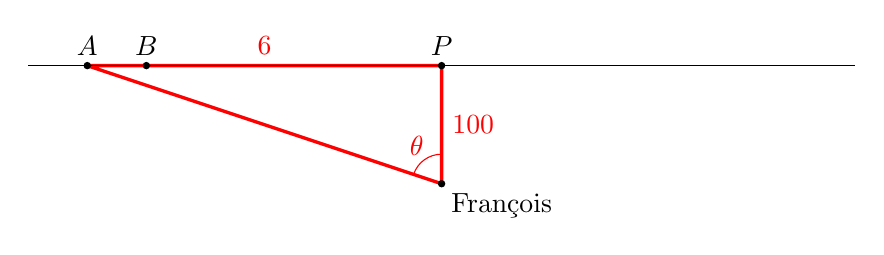
\begin{tikzpicture}[scale=0.75]
          \draw[very thick, color=red] (-6, 0) -- node[midway,
          anchor=south]{6} (0, 0) --
          node[midway, anchor=west]{100} (0, -2) --
          (-6, 0);
          \draw[color=red] (0, -1.5) node[xshift=-0.9em, yshift=0.3em]{$\theta$} arc (90:{90+atan(3)}:0.5);
          \draw (-7, 0) -- (7, 0);
          \filldraw (0, 0) node[above] {$P$} circle (1.5pt);
          \filldraw (0, -2) node[anchor=north west] {Fran\c{c}ois} circle (1.5pt);
          \filldraw (-5, 0) node[above]{$B$} circle (1.5pt);
          \filldraw (-6, 0) node[above]{$A$} circle (1.5pt);
        \end{tikzpicture}
      \end{center}
      From this, we can see that $\tan \theta = \frac{6}{100}$.  Since
      $\theta$ is between $0$ and $\frac{\pi}{2}$, that means we can
      express $\theta$ as $\boxed{\arctan \left( \frac{6}{100} \right)}$. 
    \end{solution}

  \item \label{francois-rope-optimization-angle}
    \begin{problem}[\vfill\newpage]
      Fran\c{c}ois' angle of view of the two knots is defined to be the
      angle between the two dashed lines shown below.
      \begin{center}
        \begin{tikzpicture}[scale=0.75]
          \draw (-7, 0) -- (7, 0);
          \filldraw (0, 0) node[above] {$P$} circle (1.5pt);
          \filldraw (0, -2) node[anchor=west] {Fran\c{c}ois} circle (1.5pt);
          \filldraw (-5, 0) node[above]{$B$} circle (1.5pt);
          \filldraw (-6, 0) node[above]{$A$} circle (1.5pt);
          \draw[dashed] (-5, 0) -- (0, -2) -- (-6, 0);
        \end{tikzpicture}
      \end{center}
      Write an expression for his angle of view of the two knots. 
    \end{problem}

    \begin{solution}
      Using our answer from \ref{francois-rope-optimization-prep}, the
      angle of view is $\arctan \left( \frac{6}{100} \right)$ minus the
      angle shown below:
      \begin{center}
        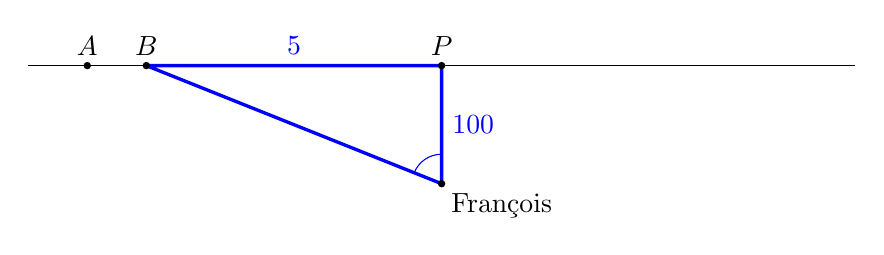
\begin{tikzpicture}[scale=0.75]
          \draw[very thick, color=blue] (-5, 0) -- node[midway,
          anchor=south]{5} (0, 0) --
          node[midway, anchor=west]{100} (0, -2) --
          (-5, 0);
          \draw[color=blue] (0, -1.5) arc (90:{90+atan(2.5)}:0.5);
          \draw (-7, 0) -- (7, 0);
          \filldraw (0, 0) node[above] {$P$} circle (1.5pt);
          \filldraw (0, -2) node[anchor=north west] {Fran\c{c}ois} circle (1.5pt);
          \filldraw (-5, 0) node[above]{$B$} circle (1.5pt);
          \filldraw (-6, 0) node[above]{$A$} circle (1.5pt);
        \end{tikzpicture}
      \end{center}
      By the same reasoning as in \ref{francois-rope-optimization-prep},
      the indicated angle is $\arctan \left( \frac{5}{100} \right)$, so
      the angle of view is $\boxed{\arctan \left( \frac{6}{100} \right) -
        \arctan \left( \frac{5}{100} \right)}$. 
    \end{solution}

  \item 

    \begin{problem}[\newpage]
      Fran\c{c}ois walks directly toward point $P$.  At what distance from
      the rope is his angle of view of the two knots the greatest?
    \end{problem}

    \begin{solution}
      \ideas{This is an optimization problem, so we start by identifying
        our goal.} 

      \highlight{\textbf{Goal:} Maximize Fran\c{c}ois' angle of view.} 

      \ideas{Next, we write a formula for the thing we're trying to maximize
        (angle of view).  To do this, we'll need to define some variables.}

      \highlight{\textbf{Define variables:} Let $A$ be the angle of view
        and $x$ be Fran\c{c}ois' distance from the rope.}

      \highlight{\textbf{Formula for thing we're trying to maximize:}
        Using the same reasoning as in
        \ref{francois-rope-optimization-angle}, $\displaystyle A = \arctan
        \left( \frac{6}{x} \right) - \arctan \left( \frac{5}{x} \right)$.
        (Instead of being 100 meters away from the rope, Fran\c{c}ois is
        now $x$ meters from the rope.)}

      \ideas{Now, we have $A$ as a function of just one variable ($x$), so
        we can maximize.}  We want the critical points, so we should first
      find the derivative of $A(x)$:
      \begin{align*}
        A'(x) &= \frac{d}{dx} \left(\fcolorbox{red}{white}{$\displaystyle \arctan\left(\fcolorbox{blue}{white}{$\displaystyle \frac{6}{x} $}\right)$}\right)-\frac{d}{dx} \left(\fcolorbox{red}{white}{$\displaystyle \arctan\left(\fcolorbox{blue}{white}{$\displaystyle \frac{5}{x} $}\right)$}\right) \\
        &= \frac{1}{1 + \left( \frac{6}{x} \right)^2} \cdot (-6x^{-2}) -
        \frac{1}{1 + \left( \frac{5}{x} \right)^2} \cdot (-5x^{-2}) \\
        &= \frac{1}{1 + \frac{36}{x^2}} \cdot \frac{-6}{x^2} - \frac{1}{1
          + \frac{25}{x^2}} \cdot \frac{-5}{x^2} \\
      &= - \frac{6}{x^2 + 36} + \frac{5}{x^2 + 25} \\
      &= \frac{-6(x^2 + 25) + 5 (x^2 + 36)}{(x^2 + 25)(x^2 + 36)} \\
      &= \frac{30 - x^2}{(x^2 + 25)(x^2 + 36)}
      \end{align*}
      This is never undefined, and it's 0 when $x^2 = 30$, i.e., when $x =
      \pm \sqrt{30}$.  Since $x$ represents a distance, it must be
      positive, so the only relevant critical number is $x = \sqrt{30}$.

      \ideas{But wait, we're not done yet!  We've found a critical point,
        but we still need to determine whether it's the absolute maximum.}
      Let's use the First Derivative Test to see if this is really a
      maximum.  We test points to get the following sign chart:
      \begin{center}
        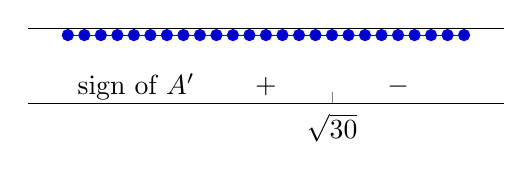
\begin{tikzpicture}
          \begin{axis}[axis y line=none, x axis line style={-}, xtick={5.47723}, xticklabels={$\sqrt{30}$}, ymin=-2, height=1in, width=3in]
            \addplot+[domain=-5.47723:10.9545]{0};
            \draw (axis cs: -5.47723, -1.5) node[right] {sign of $A '$};
            \draw (axis cs: 2.73861, -1.5) node{$+$};
            \draw (axis cs: 8.21584, -1.5) node{$-$};
          \end{axis}
        \end{tikzpicture}
      \end{center}
      For example, $A'(1) = \frac{29}{26 \cdot 37} > 0$ and $A'(10) =
      \frac{-70}{125 \cdot 136} < 0$.  So, $x = \sqrt{30}$ indeed gives
      the maximum angle, and Fran\c{cois} should stand \fbox{$\sqrt{30}$
        feet away} to get the maximum viewing angle.
    \end{solution}

  \end{enumerate}

\item 

  %\emph{Modeling.}  
  
  The following parts are unrelated.

  \begin{enumerate}
  
  \item 

    Firehiwot is growing a mold for an experiment.  The mold naturally
    grows at a rate proportional to its own size.  
    \begin{enumerate}
    \item

      \begin{problem}[\vfill]
        After two hours, the mold has grown to three times its original
        size.  If $M(t)$ is the size of the mold (in mg) at time $t$
        (where $t$ is measured in hours), write a differential equation
        that models the situation.  (Your differential equation should
        \emph{not} include any unknown constants.) 
      \end{problem}

      \begin{solution}
        Since the mold naturally grows at a rate proportional to its own
        size, we know that $\frac{dM}{dt} = kM$.  However, we are told
        that our differential equation should not include any unknown
        constants, so we need to find a value for $k$.

        We are told that the mold grows to three times its original size
        in 2 hours; that is, $M(2) = 3 M(0)$.  To use this, we need a
        formula for $M(t)$; fortunately, we know that the solution of our
        differential equation $\frac{dM}{dt} = kM$ is $M(t) = C e^{kt}$.
        Using this, our equation
        \begin{align*}
          M(2) &= 3 M(0) \\
          \shortintertext{can be rewritten as}
          C e^{2k} &= 3 C \\
          e^{2k} &= 3 \\
          \shortintertext{And now we can solve for $k$:}
          2k &= \ln 3 \\
          k &= \frac{\ln 3}{2}
        \end{align*}
        So, the differential equation we want is $\boxed{ \frac{dM}{dt} =
          \frac{\ln 3}{2} M}$. 
      \end{solution}

    \item
      \begin{problem}[\vfill]
        Once the mold has gotten large enough, Firehiwot starts removing
        10 mg of mold each hour to perform tests on it.  If $M(t)$ is the
        size of the mold (in mg) at time $t$ (where $t$ is measured in
        hours), write a differential equation that models this new
        situation.  (Model Firehiwot's harvesting of mold as happening
        continuously.) 
      \end{problem}

      \begin{solution}
        We must factor two rates into our differential equation:
        \begin{enumerate}[label=\arabic*.]
        \item The mold is growing at a rate proportional to its own size.
          As we figured out in the previous part, this rate can be
          expressed as $\frac{\ln 3}{2} M$.
        \item Firehiwot removes 10 mg of the mold per hour.  This rate is
          a constant, 10 mg/hr. 
        \end{enumerate}
        We put these together as
        \[ \frac{dM}{dt} = (\text{rate of growth of mold}) - (\text{rate
          at which mold is being removed}),\] or $\boxed{ \frac{dM}{dt} =
          \frac{\ln 3}{2} M - 10}$.
      \end{solution}

    \end{enumerate}

  \item \label{sinusoid-hours-of-daylight} 
    \begin{problem}[\vfill\newpage]
      At a particular line of latitude, the longest day of the year is
      June 21st with 14 hours of daylight, and the shortest day of the
      year is December 21st with 10 hours of daylight.  The relationship
      between the length of the day and the day of the year can be
      approximated by a sinusoidal function. Let $L(t)$ be the number of
      hours of daylight at time $t$, where $t$ is measured in months and
      $t = 0$ corresponds to September 21st, the autumnal equinox.  Write
      a function for $L(t)$.
    \end{problem}

    \begin{solution}
      December 21 corresponds to $t = 3$, while June 21 corresponds to $t
      = 9$.  So, here's a sketch of $L(t)$:
      \begin{center}
        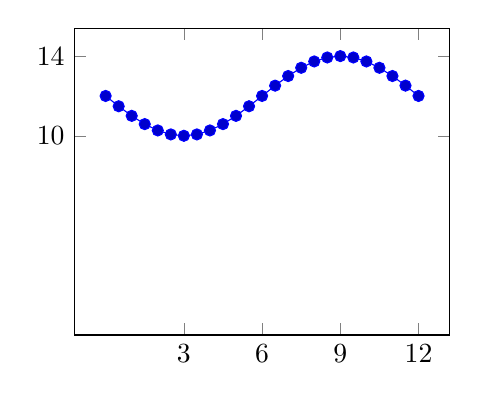
\begin{tikzpicture}
          \begin{axis}[ymin=0, ytick={10, 14}, width=2.5in, xtick={3, 6,
              9, 12}]
            \addplot+[domain=0:12] {-2*sin(pi/6*deg(x))+12};
          \end{axis}
        \end{tikzpicture}
      \end{center}
      To model this, it's helpful to find the amplitude, midline value,
      and period.  The period is 12 months, since we are looking at a
      yearly cycle.  The amplitude is half of the difference between the
      highest value (14) and lowest value (10), so the amplitude is 2.
      The midline value is the value half-way between 10 and 14, which is
      12.

      Based on our sketch, it makes most sense to model with a vertically
      flipped sine function since, at $t = 0$, the function we're modeling
      is at its midline value and decreasing.  So, the model is $L(t) = -2
      \sin \left( \frac{2 \pi}{12} t \right) + 12$, which simplifies to
      $\boxed{-2 \sin \left( \frac{\pi}{6} t \right) + 12}$.
    \end{solution}

  \end{enumerate}

\item
  \label{curve-sketching-with-sub-2}

  In this problem, you'll look at $\displaystyle f(x) =
  \frac{x}{e^{x^2}}$. 

  \begin{enumerate}

  \item
    \begin{problem}[0.5in]
      What is the domain of $f$?
    \end{problem}

    \begin{solution}
      $e^{x^2}$ is defined for all $x$ and is never 0, so $f(x)$ is
      defined for \fbox{all real numbers}. 
    \end{solution}

  \item
    \begin{problem}[\vfill]
      Is $f(x)$ an even function, an odd function, or neither?
    \end{problem}

    \begin{solution}
      \ideas{To test this, we should look at $f(-x)$.}
      \begin{align*}
        f(-x) &= \frac{-x}{e^{(-x)^2}} \\
        &= - \frac{x}{e^{x^2}} \\
        &= - f(x)
      \end{align*}
      So, $f$ \fbox{is an odd function}. 
    \end{solution}

  \item \label{curve-sketching-with-sub-2-increasing}
    \begin{problem}[\stretch{2}]
      For what values of $x$ (in the domain of $f$) is $f(x)$ increasing? 
    \end{problem}

    \begin{solution}
      \ideas{To answer this, let's make a sign chart for $f'$, since we
        know that the sign of $f'$ tells us whether $f$ is increasing or
        decreasing.}  First, we'll calculate $f'$:
      \begin{align*}
        f'(x) &= \frac{d}{dx}
        \left(\fcolorbox{green}{white}{$\displaystyle  x$}\cdot
          \fcolorbox{green}{white}{$\displaystyle  e^ { -x^ { 2} }
            $}\right) \\
        &= x\cdot \frac{d}{dx}
        \left(\fcolorbox{red}{white}{$\displaystyle e^ {
              \fcolorbox{blue}{white}{$\displaystyle -x^ { 2} $}}
            $}\right)+ e^ { -x^ { 2} }  \\ 
        &= x \cdot e^ { -x^ { 2} } \left(-2 x\right)+ e^
        { -x^ { 2} } \\
        &= e^{-x^2} \left(1 - 2x^2 \right)
      \end{align*}
      $f'$ is never undefined, so let's find where $f'(x) = 0$:
      \begin{align*}
        e^{-x^2} \left(1 - 2x^2 \right) &= 0 \\
        \intertext{$e^{-x^2}$ is never 0, so we need}
        1 - 2x^2 &= 0 \\
        1 &= 2x^2 \\
        \frac{1}{2} &= x^2 \\
        x &= \pm \frac{1}{\sqrt{2}}
      \end{align*}
      Now, we can make a sign chart for $f'$:
      \begin{center}
        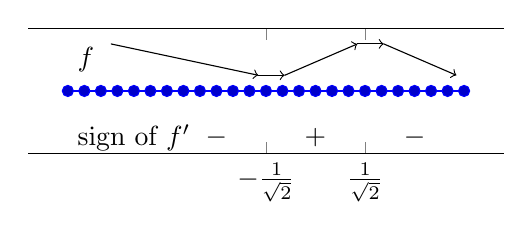
\begin{tikzpicture}
          \begin{axis}[axis y line=none, x axis line style={-}, xtick={-0.707107, 0.707107}, xticklabels={$-\frac{1}{\sqrt{2}}$, $\frac{1}{\sqrt{2}}$}, ymin=-2, ymax=2, height=1.25in, width=3in]
            \addplot+[domain=-3.53553:2.12132]{0};
            \draw (axis cs: -3.53553, -1.5) node[right] {sign of $f'$};
            \draw (axis cs: -3.53553, 1) node[right] {$f$};
            \draw (axis cs: -1.41421, -1.5) node{$-$};
            \draw[->, xshift=2pt] (axis cs: -3, 1.5) -- (axis cs: -0.895669, 0.5);
            \draw (axis cs: 0., -1.5) node{$+$};
            \draw[->, xshift=2pt] (axis cs: -0.518545, 0.5) -- (axis cs: 0.518545, 1.5);
            \draw (axis cs: 1.41421, -1.5) node{$-$};
            \draw[->, xshift=2pt] (axis cs: 0.895669, 1.5) -- (axis cs: 1.93276, 0.5);
            \draw[->, xshift=2pt] (axis cs: -0.895669, 0.5) -- (axis cs: -0.518545, 0.5);
            \draw[->, xshift=2pt] (axis cs: 0.518545, 1.5) -- (axis cs: 0.895669, 1.5);
          \end{axis}
        \end{tikzpicture}
      \end{center}
      So, $f$ is increasing on $\boxed{\left( - \frac{1}{\sqrt{2}},
          \frac{1}{\sqrt{2}} \right)}$. 
    \end{solution}

  \item 
    \begin{problem}[\vfill\newpage]
      Find $\displaystyle \lim_{x \to \infty} f(x)$.
    \end{problem}

    \begin{solution}
      We are asked to find $\displaystyle \lim_{x \to \infty}
      \frac{x}{e^{x^2}}$.  As $x \to \infty$, both the numerator and
      denominator $\to \infty$, so we have a limit of the indeterminate
      form $\frac{\infty}{\infty}$, and we can use L'H\^opital's Rule:
      \begin{align*}
        \lim_{x \to \infty} \frac{x}{e^{x^2}} &
        \stackrel{\text{L'H}}{=} \lim_{x \to \infty} \frac{1}{2x e^{x^2}}
        \\
        \intertext{Now, the denominator $\to \infty$, while the numerator
          is just 1, so the entire limit is }
        &= \boxed{0}
      \end{align*}
    \end{solution}

  \item
    \begin{problem}[\vfill]
      Does $f(x)$ have an absolute maximum value on $(-\infty, \infty)$?
      If so, at what $x$-value(s) does the absolute maximum occur?
    \end{problem}

    \begin{solution}
      The sign chart we made in
      \ref{curve-sketching-with-sub-2-increasing} is helpful but does not
      answer the question; from the sign chart, we can see that $f(x)$
      \emph{might} have an absolute maximum at $x = \frac{1}{\sqrt{2}}$,
      but it's also possible that the graph of $f(x)$ is higher when $x$
      is very negative.  To figure out what's really going on, we need to
      compare $f \left( \frac{1}{\sqrt{2}} \right)$ with $\displaystyle
      \lim_{x \to -\infty} f(x)$:
      \[ f \left( \frac{1}{\sqrt{2}} \right) = \frac{1 /
        \sqrt{2}}{e^{1/2}} = \frac{1}{\sqrt{2e}}\]
      We could compute $\displaystyle \lim_{x \to -\infty} f(x)$ directly,
      or we could use symmetry: since $f(x)$ is odd and we already found
      that $\displaystyle \lim_{x \to \infty} f(x) = 0$, it must be the
      case that $\displaystyle \lim_{x \to -\infty} f(x) = 0$ as well.
      Therefore, the graph of $f(x)$ is higher at $x = \frac{1}{\sqrt{2}}$
      than it is as $x \to -\infty$, and $f(x)$ has an absolute maximum
      value at $\boxed{x = \frac{1}{\sqrt{2}}}$.       
    \end{solution}

  \item
    \begin{problem}[\vfill]
      Sketch a rough graph of $f(x)$.  Your graph should reflect what you
      have done in this problem, but you do \textbf{not} need to
      accurately show the concavity of $f(x)$. 
    \end{problem}

    \begin{solution}
      \begin{center}
        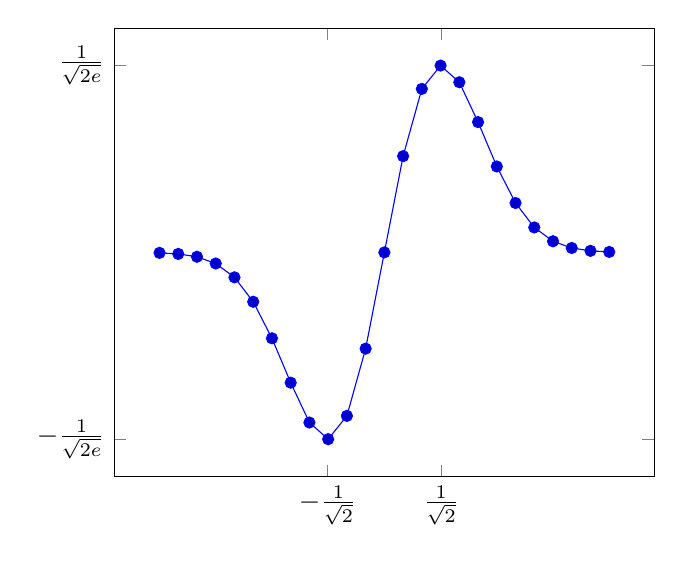
\begin{tikzpicture}
          \begin{axis}[xtick={-0.707, 0.707},
            xticklabels={$-\frac{1}{\sqrt{2}}$, $\frac{1}{\sqrt{2}}$},
            ytick={-0.429, 0.429}, yticklabels={$-\frac{1}{\sqrt{2e}}$,
              $\frac{1}{\sqrt{2e}}$}] 
            \addplot+[domain=-2.8:2.8]{x/e^(x^2)};
          \end{axis}
        \end{tikzpicture}
      \end{center}
    \end{solution}

    \begin{grading}
      The key features your graph should have are:
      \begin{itemize}
      \item It's an odd function.
      \item It's decreasing on $\left(-\infty, - \frac{1}{\sqrt{2}}
        \right)$, increasing on $\left( - \frac{1}{\sqrt{2}},
          \frac{1}{\sqrt{2}} \right)$, and decreasing on $\left(
          \frac{1}{\sqrt{2}}, \infty \right)$.
      \item As $x \to \pm \infty$, $f(x) \to 0$.
      \end{itemize}
    \end{grading}

  \item
    \begin{problem}[\vfill\newpage]
      Find the signed area under $y = f(x)$ from $x = -3$ to $x = 2$.
    \end{problem}

    \begin{solution}
      We are asked to find $\displaystyle \int_{-3}^{2} f(x)\,dx =
      \int_{-3}^{2} \frac{x}{e^{x^2}}\,dx$.  Let's rewrite the integrand as
      $x e^{-x^2}$ and substitute \sub{$u = -x^2$}.  Then, $du = -2x\,dx$,
      so \subd{$- \frac{du}{2} = x\,dx$}. 
      \begin{align*}
        \int_{-3}^{2} \subd{x} e^{\sub{-x^2}}\,\subd{dx} &= \int_{-9}^{-4}
        e^\sub{u} \left( \subd{- \frac{du}{2}} \right)  \\
        &= - \frac{1}{2} e^u \Big|_{-9}^{-4} \\
        &= \boxed{- \frac{1}{2} e^{-4} + \frac{1}{2} e^{-9}}
      \end{align*}
      \begin{checkanswer}
        From our graph, we can see that this signed area should be negative
        (and our calculation is consistent with that).
      \end{checkanswer}
    \end{solution}

  \end{enumerate}

\item \label{sinusoid-woods-hole}

  The water level at Woods Hole Oceanographic Institution naturally rises
  and falls due to tides.  Suppose the height of the water at time $t$
  ($t$ in hours) is given by $\displaystyle h(t) = -2 \sin \left( \frac{2
      \pi}{11} t \right) + 3$ feet.
  \begin{enumerate}
  \item \label{sinusoid-woods-hole-graph}
    \begin{problem}[\vfill]
      Sketch $h(t)$ on $[0, 24]$.  Please label your graph clearly, so
      that we can see precisely where the local extrema occur. 
    \end{problem}

    \begin{solution}
      We get the graph of $h(t)$ by starting with the graph of $\sin t$,
      stretching it horizontally so that its period is 11, flipping it
      vertically and stretching it so that its amplitude is 2, and moving
      it up 3:
      \begin{center}
        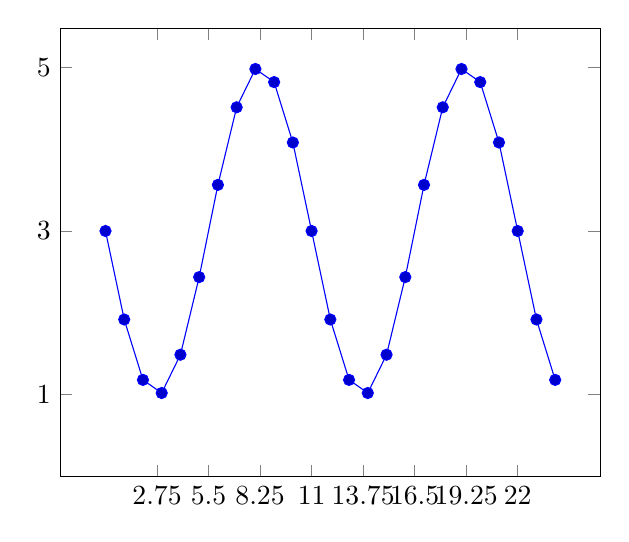
\begin{tikzpicture}
          \begin{axis}[xtick={2.75, 5.5, ..., 22}, ytick={1, 3, 5}, ymin=0]
            \addplot+[domain=0:24] { -2*sin(deg(2*pi/11*x))+3}; 
          \end{axis}
        \end{tikzpicture}
      \end{center}
    \end{solution}

  
  \item
    \begin{problem}[\vfill]
      Between $t = 0$ and $t = 33$, how many times will the water level be
      exactly $2.5$ feet?  Explain briefly. 
    \end{problem}

    \begin{solution}
      If we imagine extending our graph in \ref{sinusoid-woods-hole-graph}
      to $[0, 33]$, we would have three complete periods, and we can see
      that there will be \fbox{6} times at which the water level is
      exactly 2.5 feet:
      \begin{center}
        \begin{tikzpicture}
          \begin{axis}[xtick={11, 22, 33}, ytick={1, 2.5, 3, 5},
            ymin=0, width=4in, height=2in, cycle list name=mycolor]
            \addplot+[domain=0:33] { -2*sin(deg(2*pi/11*x))+3};
            \addplot+[domain=0:33] {2.5};
          \end{axis}
        \end{tikzpicture}
      \end{center}      
    \end{solution}
    \newpage
\item
    \begin{problem}[\vfill]
      What are the first two times after $t = 0$ at which the water level
      is $4$ feet?
    \end{problem}

    \begin{solution}
      We are looking for the first two times after $t = 0$ at which
      \begin{align*}
        -2 \sin \left( \frac{2 \pi}{11} t \right) + 3 &= 4 \\
        -2 \sin \left( \frac{2 \pi}{11} t \right) &= 1 \\
        \sin \left( \frac{2 \pi}{11} t \right) &= - \frac{1}{2} \\
        \intertext{Let's substitute $u = \dfrac{2 \pi}{11} t$.  We are
          interested in $t > 0$, which corresponds to $u > 0$.}
        \sin (u) &= -\frac{1}{2} \\
        \intertext{The two smallest positive values of $u$ such that $\sin
          u = - \frac{1}{2}$ are }
        u &= \frac{7 \pi}{6}, \frac{11 \pi}{6} \\
        \intertext{Now, we go back and solve for $t$: since $u = \frac{2
            \pi}{11} t$, $t = \frac{11}{2 \pi} u$:}
        t &= \boxed{\frac{77}{12}, \frac{121}{12}}
      \end{align*}
      \begin{checkanswer}
        From our graph, we can see that the values we were looking for
        should be between 5.5 and 11, so our answer seems reasonable.  We
        can also plug our answers back into $h(t)$ to check: for instance,
        $h \left( \frac{77}{12} \right) = -2 \sin \left( \frac{7 \pi}{6}
        \right) + 3 = 4$, as we wanted.
      \end{checkanswer}
    \end{solution}
  \item
    \begin{problem}[\vfill\newpage]
      What are the first two times after $t = 0$ at which the water level
      is $2.5$ feet?  
    \end{problem}

    \begin{solution}
      We are looking for the first two times after $t = 0$ at which
      \begin{align*}
        -2 \sin \left( \frac{2 \pi}{11} t \right) + 3 &= 2.5 \\
        -2 \sin \left( \frac{2 \pi}{11} t \right) &= -0.5 \\
        \sin \left( \frac{2 \pi}{11} t \right) &= \frac{1}{4} \\
        \intertext{Let's substitute $u = \dfrac{2 \pi}{11} t$.  We are
          interested in $t > 0$, which corresponds to $u > 0$.}
        \sin (u) &= \frac{1}{4} \\
        \intertext{Now, we don't know any ``nice'' angles whose sine is
          $\dfrac{1}{4}$, so we use $\arcsin$:}
        u &= \arcsin \frac{1}{4}, \pi - \arcsin \frac{1}{4}
        \intertext{Now, we go back and find $t$: since 
          $u = \dfrac{2 \pi}{11} t$, $t = \dfrac{11}{2 \pi} u$:}
        t &= \boxed{\frac{11}{2 \pi} \arcsin \left( \frac{1}{4} \right),
          \frac{11}{2 \pi} 
          \left[ \pi - \arcsin \left( \frac{1}{4} \right) \right]}
      \end{align*}

    \end{solution}
  \end{enumerate}

\item \label{spring2010-mb-final-review-2-mystery}

  Suppose $f$ is an unknown function which is continuous and always
  increasing on $[-3, 7]$.  You also know that $f(1) = 0$. For each
  statement below, decide if the statement must be true, must be false, or
  if you don't have enough information to be sure.  Circle your choice,
  and explain your reasoning briefly.

  \providecommand{\answerblock}{}
  \renewcommand{\answerblock}[1]{%
    \begin{center}
      \solonly{\maybecircle[#1=1]}{True} \quad
      \solonly{\maybecircle[#1=2]}{False} \quad
      \solonly{\maybecircle[#1=3]}{Not enough info}
    \end{center}
    \pspace{\vfill}
  }

  \begin{enumerate}

  \item
    \begin{problem}
      If $R_n$ is the right-hand sum with $n$ rectangles which
      approximates $\displaystyle \int_{-3}^7 f(x)\,dx$, then
      $\displaystyle \lim_{n \to \infty} R_n$ is an overestimate of
      $\displaystyle \int_{-3}^7 f(x)\,dx$ (that is, $\displaystyle \lim_{n
        \to \infty} R_n > \int_{-3}^7 f(x)\,dx$).
    \end{problem}

    \answerblock{2}

    \begin{solution}
      The limit $\displaystyle \lim_{n \to \infty} R_n$ is \textbf{equal}
      to $\displaystyle \int_{-3}^7 f(x)\,dx$: that's the definition of
      the definite integral!
    \end{solution}

  \item \label{spring2010-final-review-2-mystery-b}
    \begin{problem}
      If $\displaystyle A(x) = \int_{2}^x f(t) \,dt$, then the derivative
      of $A(x)$ is $f(x)$.
    \end{problem}

    \answerblock{1}

    \begin{solution}
      This is what Part 1 of the Fundamental Theorem of Calculus says.
    \end{solution}

  \item
    \begin{problem}
      If $\displaystyle B(x) = \int_{-3}^7 f(t) \,dt$, then the derivative
      of $B(x)$ is $f(x)$.
    \end{problem}

    \answerblock{2}

    \begin{solution}
      Here, $B(x)$ is constant, so $B'(x) = 0$. 
    \end{solution}

  \item
    \begin{problem}
      If $\displaystyle C(x) = \int_x^2 f(t)\,dt$, then the derivative of
      $C(x)$ is $f(2)$.
    \end{problem}

    \answerblock{2}

    \begin{solution}
      By properties of integrals, $C(x) = - A(x)$, where $A(x)$ is the
      function in \ref{spring2010-final-review-2-mystery-b}.  Therefore,
      $C'(x) = - A'(x) = -f(x)$. 
    \end{solution}

  \item

    \begin{problem}
      If $\displaystyle F(x) = \int_{-3}^x f(t) \,dt$ and $\displaystyle
      G(x) = \int_{0}^x f(t) \,dt$, then the graph of $G(x)$ is a vertical
      shift downward of the graph of $F(x)$ (that is, we can shift the
      graph of $F(x)$ down to get the graph of $G(x)$).
    \end{problem}

    \answerblock{2}

    \begin{solution}
      First, notice that $F(x) = {}_{-3} A_f(x)$, and $G(x) =
        {}_0 A_f(x)$, so $F(x)$ and $G(x)$ are both area functions for
        $f$, and they must differ by a constant.  We want to know about
        the sign of this constant, so let's look at the difference $F(x) -
        G(x)$:
      \begin{align*}
        F(x) - G(x) &= \int_{-3}^x f(t)\,dt - \int_{0}^x f(t)\,dt \\
        &= \int_{-3}^0 f(t)\,dt
      \end{align*}
      We are told that $f$ is increasing on $[-3, 7]$ and that $f(1) = 0$,
      so $f$ must be negative on $[-3, 0]$.  Therefore, $\displaystyle
      \int_{-3}^0 f(t)\,dt$ must be negative.  So, $F(x) - G(x)$ is a
      negative number, which means that $F(x)$ is a vertical shift
      \emph{downward} of $G(x)$.
    \end{solution}

  \item
    \begin{problem}
      If $H (x) = \displaystyle \int_{1}^x f(t) \,dt$, then $H(x)$ is
      increasing on $[-3, 7]$.
    \end{problem}

    \answerblock{2}

    \begin{solution}
      $H$ is increasing when $H' > 0$; since $H(x)$ is just
        the area function $_1 A_f$, $H' = f$, which is $> 0$ only for $x >
        1$.

    \end{solution}

  \end{enumerate}
  \pspace{\newpage}
  \probonly{\newpage}

\item \label{spring2011-1b-midterm1-snow-density-modified} %\finishexam 
  % based on David Ayala's problem 

  Recently, the state of Illinois experienced a severe snow storm.  The
  mayors of two different cities are trying to determine how much snow
  fell on their cities during the storm.

  \begin{enumerate}
  \item \label{spring2011-midterm1-snow-density-circle}
    \begin{problem}[2.65in]
      City A is circular with a radius of 5 km, and the density of snow
      from the storm is given by $\rho(x)$ kg/km$^2$, where $x$ represents
      distance from the center of the city.  Write an integral giving the
      total amount of snow that fell on City A.

      Please include a sketch that shows how you are slicing. 
    \end{problem}

    \begin{solution}
      Since the density of snow varies with distance from the center of
      the city, we must slice in concentric rings around the city center
      (within a single ring, every point is approximately the same
      distance from the center of the city, so every point has
      approximately the same density of snow).  Note that $x = 0$ at the
      center of the city and $x = 5$ at the edge of the city, so we're
      slicing the interval $[0, 5]$.  Let's look at the $k$-th slice:
      \begin{center}
        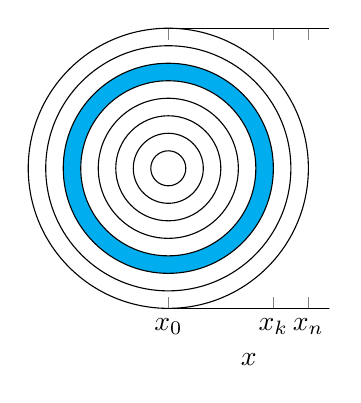
\begin{tikzpicture}
          \begin{axis}[x=0.007in, y=0.007in, xmin=0, xmax=115,
            ymin=-100, ymax=100, axis on top=true, clip=false, hide y
            axis, xtick={0.1, 75, 100}, xticklabels={$x_0$, $x_k$, $x_n$},
            xlabel=$x$, tick label style={fill=none}]              
            \draw[fill=cyan, draw=none] (0, 0) circle(75); %
            \draw[fill=white, draw=none] (0, 0) circle (62.5); %
            \pgfplotsforeachungrouped \x in {12.5, 25, ..., 100.1}
            {
              \edef\temp{
                \noexpand\draw (0, 0) circle(\x);
              }
              \temp
            }              
          \end{axis}
        \end{tikzpicture}
      \end{center}
      This slice is a ring of thickness $\Delta x$ whose radius is
      approximately $x_k$, so its area is approximately $2 \pi x_k \Delta
      x$.  The density of snow in this slice is approximately $\rho(x_k)$,
      so
      \[ \text{amount of snow in $k$-th slice} \approx \rho(x_k) \cdot 2
      \pi x_k \Delta x.\] Summing over all slices and taking the limit as
      the number of slices ($n$) $\to \infty$, the total amount of snow
      that fell on City A is $\boxed{\int_0^5 \rho(x) \cdot 2 \pi x\,dx}$.
    \end{solution}

  \item 
    \begin{problem}[\vfill\newpage]
      Evaluate your integral from
      \ref{spring2011-midterm1-snow-density-circle} if $\displaystyle
      \rho(x) = \frac{1}{\sqrt{x + 4}}$.
    \end{problem}

    \begin{solution}
      We are asked to evaluate $\displaystyle \int_0^5 \frac{2 \pi
        x}{\sqrt{x + 4}}\,dx$.  Let's substitute \sub{$u = x + 4$}; then,
      \subd{$du = dx$} and \sube{$x = u - 4$}:
      \begin{align*}
        \int_0^5 \frac{2 \pi \sube{x}}{\sqrt{\sub{x + 4}}}\,\subd{dx} &=
        \int_4^9 \frac{2 \pi 
          (\sube{u - 4})}{\sqrt{\sub{u}}}\,\subd{du} \\
        &= 2 \pi \int_4^9 \left( u^{1/2} - 4 u^{-1/2} \right)\,du \\
        &= \left.  2 \pi \left( \frac{2}{3} u^{3/2} - 8 u^{1/2} \right)
        \right|_4^9 \\
        &= 2 \pi \left[ \left( \frac{2}{3} \cdot 27 - 8 \cdot 3 \right) -
          \left( \frac{2}{3} \cdot 8 - 8 \cdot 2 \right) \right] \\ 
        &= \boxed{\frac{28 \pi}{3}}
      \end{align*}
    \end{solution}

  \item 

    \begin{problem}[\newpage]
      City B is in the shape of a right triangle with sides of length 5,
      12, and 13 km.  The 5 km side lies along Lake Michigan, and the
      density of snow is given by $\rho(x)$ kg/km$^2$, where $x$
      represents distance from the lake.  Write an integral giving the
      total amount of snow that fell on City B.

      Please include a sketch that shows how you are slicing. 
    \end{problem}

    \begin{solution}      
      We are told that $x$ represents distance from the lake.  Since the
      density of snow varies with distance from Lake Michigan, we must
      slice parallel to the lake.  Note that $x = 0$ along the lake and $x
      = 12$ at the opposite end of City B, so we're slicing $[0, 12]$.  As
      usual, we focus on the $k$-th slice, and it's reasonable to
      approximate this slice as a rectangle:
      \begin{center}
        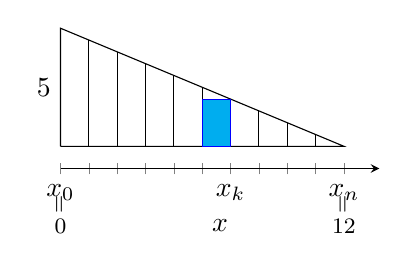
\begin{tikzpicture}
          \begin{axis}[xmin=0, xmax=4.5, ymin=0, ymax=1.8, clip=false,
            hide y axis, axis x line=bottom, xlabel=$x$, xtick={0, 0.4,
              ..., 4.01}, xticklabels={$x_0$,,,,,,$x_k$,,,,$x_n$},
            x=0.9cm, y=0.5cm]
            \begin{scope}[yshift=8pt]
              \draw (0, 0) -- node[left] {$5$} (0, 3) -- (4, 0) -- (0,
              0); %
              \pgfplotsforeachungrouped \x in {0, 0.4, ..., 4.01} {%
                \edef\temp{%
                  \noexpand\draw (\x, 0) -- (\x, {-3/4*(\x - 4)}); %
                }%
                \temp%
              }
              \draw[blue, fill=cyan] (2, 0) -- (2, 1.2) -- (2.4, 1.2) --
              (2.4, 0) -- cycle;
            \end{scope}
            \begin{scope}[font=\footnotesize]
              \draw (0, -13pt) node[rotate=90] {$=$};
              \draw (4, -13pt) node[rotate=90] {$=$};
              \draw (0, -21pt) node {$0$};
              \draw (4, -21pt) node {$12$};
            \end{scope}
          \end{axis}
        \end{tikzpicture}
      \end{center}
      We'd like to approximate the amount of snow in this slice, and we
      know:
      \begin{align*}
        \text{amount of snow in $k$-th slice} & \approx (\text{density of
          snow in $k$-th slice}) (\text{area of $k$-th slice}) \\
        \text{area of $k$-th slice} & \approx (\text{height of $k$-th
          slice})(\text{width of $k$-th slice}) \\
        & \approx (\text{height of $k$-th slice}) \Delta x \\
        \text{density of snow in $k$-th slice} & \approx \rho(x_k)
      \end{align*}
      So, the main thing we still need to do is to approximate the height
      of the $k$-th slice in terms of $x_k$.  One way to do this is to
      use similar triangles; let $h_k$ be the height of the rectangle: 
      \begin{center}
        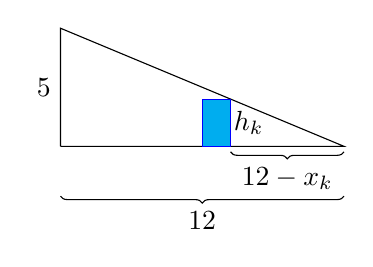
\begin{tikzpicture}
          \begin{axis}[xmin=0, xmax=4.5, ymin=0, ymax=1.8, clip=false,
            hide y axis, axis x line=bottom, x=0.9cm, y=0.5cm, xlabel=$x$,
            hide x axis] 
            \begin{scope}[yshift=8pt]
              \draw (0, 0) -- node[left] {$5$} (0, 3) -- (4, 0) -- (0,
              0); %
              \draw[blue, fill=cyan] (2, 0) -- (2, 1.2) -- (2.4, 1.2) --
              node[right, black, inner sep=1pt] {$h_k$} 
              (2.4, 0) -- cycle;
              \draw[decorate, decoration={brace, mirror}, yshift=-2pt]
              (2.4, 0) -- node[below, yshift=-2pt] {$12 - x_k$} (4, 0);
              \draw[decorate, decoration={brace, mirror}, yshift=-18pt]
              (0, 0) -- node[below, yshift=-2pt] {$12$} (4, 0);
            \end{scope}
          \end{axis}
        \end{tikzpicture}
      \end{center}
      By similar triangles, $\dfrac{5}{12} = \dfrac{h_k}{12 - x_k}$, so
      $h_k = \dfrac{5}{12} (12 - x_k)$.
      Therefore,
      \begin{align*}
        \text{amount of snow in $k$-th slice} & \approx \rho(x_k) \cdot
        \frac{5}{12} (12 - x_k) \Delta x
      \end{align*}
      Summing over all slices and taking the limit as $n \to \infty$, the
      total amount of snow in City B is $\boxed{\int_0^{12} \rho(x) \cdot
        \frac{5}{12} (12 - x) \,dx}$.
    \end{solution}

  \end{enumerate}

\end{enumerate}
\end{document}